\documentclass[conference]{IEEEtran}

\usepackage{cite}
\usepackage{amsmath,amssymb,amsfonts}
\usepackage{graphicx}
\usepackage{textcomp}
\usepackage{xcolor}
\usepackage{algpseudocode}
\usepackage{algorithm}
\usepackage{cmap}
\usepackage[T1]{fontenc}
\usepackage{lmodern}
\usepackage[english]{babel}

\def\BibTeX{{\rm B\kern-.05em{\sc i\kern-.025em b}\kern-.08em
    T\kern-.1667em\lower.7ex\hbox{E}\kern-.125emX}}
\begin{document}

\title{Implementation and Analysis of Minimal ($p$-)Absent Words in DNA Sequence}

\author{\IEEEauthorblockN{Amory ANTAO}
\IEEEauthorblockA{\textit{École Normale Supérieure Rennes}\\
Rennes, France\\
amory.antao@ens-rennes.fr}
}

\maketitle
\begin{abstract}
The identification of Minimal Absent Words (MAWs) and $p$-MAWs in DNA sequences is a major challenge in bioinformatics, particularly for understanding defense mechanisms in organisms such as CRISPR systems. This project presents the design and implementation of efficient algorithms to detect these patterns in large genomic databases.\\
After theoretical analysis, the computation of MAWs is found to have a complexity of $\mathcal{O}(n \times \text{max\_length}^2)$, while the computation of $p$-MAWs has a complexity of $\mathcal{O}(n \times \text{max\_length}^4 \times (1 + (4\gamma_p \delta_p)^{\text{max\_length}}))$, where $\gamma_p$ and $\delta_p$ are introduced parameters, and $4\gamma_p \delta_p$ remains practically below 1, thus avoiding exponential behavior. This work represents an advancement in the analysis of absent patterns in biological sequences, particularly regarding $p$-MAWs, with potential applications in genetics and molecular biology.
\end{abstract}

\section{Introduction}
\subsection{Context}
One of the recent major breakthroughs in computational biology is the discovery of the CRISPR system (Clustered Regularly Interspaced Short Palindromic Repeats) \cite{b1}, a discovery that earned E. Charpentier and J. Doudna the 2020 Nobel Prize in Chemistry for the development of the CRISPR-Cas9 genome-editing technique. This system is used by bacteria as a defense mechanism against bacterial viruses and predatory plasmids. It relies on an intern specific recognition of DNA sequences to eliminate potential threats.\\
In this context, identifying absent patterns in DNA sequences — known as the search for ``minimal absent words`` (MAWs) — is particularly relevant for understanding these defense mechanisms.
\subsection{Definition}
Before defining MAWs, it is essential to introduce the concept of the reverse complement. The reverse complement ($\text{RC}$) of a word $x$ is obtained by reversing the sequence and replacing each nucleotide base with its complement:
\begin{itemize}
\item $A\longrightarrow T$
\item $T \longrightarrow A$
\item $C \longrightarrow G$
\item $G \longrightarrow C$
\end{itemize}
This concept is critical because, in practice, when sequencing DNA, it is often impossible to know from which strand the information is extracted. To account for this bias, it is necessary to consider the reverse complement of every observed pattern.\\
An ``absent word`` (AW) of a sequence $s$ is defined as a pattern $x$ such that neither $x$ nor its reverse complement $\text{RC}(x)$ appears in $s$ as a substring.\\
However, as the size of the considered patterns increases, the number of AWs grows exponentially. To limit this combinatorial explosion, we focus on MAWs, which are minimal patterns that cannot be reduced without losing their absence property.\\
Formally, a pattern $x$ of length $|x| > 1$ is a MAW of a sequence $s$ if:
\begin{itemize}
\item $x$ is an AW of $s$, and
\item every substring $w$ of $x$, with $|w|<|x|$, is present in $s$ (or its reverse complement is present in $s$).
\end{itemize}
As an extension of this concept, it may be useful to introduce the notions of $p$-AW and $p$-MAW. For $p \in ]0, 1]$, a pattern $x$ is considered a $p$-AW of a set of sequences $\mathcal S$ if $x$ is an AW in at least $p \cdot |\mathcal S|$ sequences $s \in \mathcal S$. Similarly, $x$ is a $p$-MAW of $\mathcal S$ if it is a $p$-AW of $\mathcal S$ and all of its substrings $w$ that are different from $x$ are not $p$-AWs of $\mathcal S$.
\subsection{First Examples}
Let’s take two simple examples on the alphabet $\{a, b\}$ to illustrate these definitions.These examples are simplified because they use a smaller alphabet and do not consider reverse complements, but they will help us clearly understand the concepts discussed.
\paragraph{Example 1}
Consider the sequence $s = abaaba$. The pattern $bab$ does not appear in $s$, making it an AW of $s$. Furthermore, the substrings $ba$, $ab$, $a$, and $b$ are all present in $s$, which allows us to conclude that $bab$ is a MAW of $s$.
\paragraph{Example 2}
Now, consider the set of sequences $\mathcal S = {abbaa, bbb, bbba}$ with $p = 0.5$.\\
In this case, a pattern must be absent from at least two sequences ($0.5 \times 3 = 1.5$).\\
The pattern $bbbb$ does not appear in any of the sequences in $\mathcal S$. Therefore, it is a $p$-AW. Moreover, the substrings of $bbbb$ ($b$, $bb$, $bbb$) appear in at least two sequences in $\mathcal S$, allowing us to conclude that $bbbb$ is a $p$-MAW.
\subsection{Important Remarks}
From the previous examples, two key observations can be made:
\begin{itemize}
\item To check whether a pattern $x = x_1x_2\ldots x_n$ is a MAW of a sequence $s$, it is sufficient to verify that:
\begin{itemize}
\item $x$ is an AW of $s$, and
\item the sub-patterns $x'=x_2\ldots x_n$ and $x'' = x_1\ldots x_{n-1}$ are not AWs of $s$.
\end{itemize}
This is because any substring $w$ of $x$ such as $w\neq x$, can be expressed as a substring of either $x'$ or $x''$. If both $x'$ and $x''$ are not AWs of $s$, then none of the substrings of $x$ will be AWs either.
\item A pattern can be a $p$-MAW without being a MAW of any individual sequence in $\mathcal S$.\\
For instance, consider the case of $\mathcal S = {s_1=abbaa, s_2=bbb, s_3=bbba}$ with $p = 0.5$, and the pattern $x = bbba$:
\begin{itemize}
\item $x$ is not a MAW of $s_1$ because $bbb$ is an AW of $s_1$
\item $x$ is not a MAW of $s_2$ because $a$ is an AW of $s_2$
\item $x$ is not an AW of $s_3$ because $x = s_3$
\end{itemize}
However, $x$ is a $p$-AW of $\mathcal S$ because it is absent from two sequences: $s_1$ and $s_2$.
Moreover, $bbb$ is not an $p$-AW of $\mathcal S$ because it is in $s_2$ and $s_3$, and $bba$ is not an $p$-AW of $\mathcal S$ because it is in $s_1$ and $s_2$.\\
Therefore, $x$ is a $p$-MAW of $\mathcal S$.
\end{itemize}
\subsection{Objectives}
The main objective of this work is to design and implement efficient algorithms to identify MAWs and $p$-MAWs in a set of DNA sequences.\section{Methods: Finding Limited-Length MAWs}
\subsection{General Algorithm}
The general outline of the algorithm is as follows:
\begin{algorithm}
\caption{Find\_MAWs(S, max)}
\begin{algorithmic}[1]
\Require S : DNA sequence of length $n$
\Require max : maximum MAW length
\Ensure $MAWs$ : list of minimal absent words

\State $sa \gets \text{SuffixArray}(S)$
\State $st \gets \text{SuffixTree}(S)$
\State $MAWs \gets \emptyset$

\State $potMAWs \gets \text{PotentialMAWs}(\text{S}, sa, \text{max}))$
\ForAll{$maw \in potMAWs$}
	\If{$\text{Verify}(\text{S}, st, maw, \text{max})$}
        \State $MAWs \gets MAWs \cup \{maw\}$
    \EndIf
\EndFor

\State \Return $MAWs$
\end{algorithmic}
\end{algorithm}

The algorithm is divided into several parts:
\begin{itemize}
\item Building the suffix array and suffix tree of the input DNA sequence
\item Searching for potential MAWs between successive pairs of suffixes in the suffix array
\item Verifying whether the potential MAWs are actual minimal absent words
\end{itemize}
\subsection{Suffix Array Construction}
The suffix array is a data structure that lists all suffixes of a sequence, sorted in lexicographical order. Each suffix is represented by its starting index in the original sequence.
\paragraph{Example}
For the sequence $s = abaaba$, the different suffixes are:\\
\begin{table}[htbp]
\caption{List of suffixes of $s$}
\begin{center}
\begin{tabular}{|c|c|}
\hline
\textbf{Suffix} & \textbf{Index}\\
\hline
$abaaba$ & $0$\\
\hline
$baaba$ & $1$\\
\hline
$aaba$ & $2$\\
\hline
$aba$ & $3$\\
\hline
$ba$ & $4$\\
\hline
$a$ & $5$\\
\hline
\end{tabular}
\end{center}
\end{table}

\begin{table}[htbp]
\caption{List of suffixes of $s$ sorted lexicographically}
\begin{center}
\begin{tabular}{|c|c|}
\hline
\textbf{Suffix} & \textbf{Index}\\
\hline
$a$ & $5$\\
\hline
$aaba$ & $2$\\
\hline
$aba$ & $3$\\
\hline
$abaaba$ & $0$\\
\hline
$ba$ & $4$\\
\hline
$baaba$ & $1$\\
\hline
\end{tabular}
\end{center}
\end{table}
\begin{table}[htbp]
\caption{Suffix array of $s$}
\begin{center}
\begin{tabular}{|c|c|c|c|c|c|}
\hline
$5$ & $2$ & $3$ & $0$ & $4$ & $1$\\
\hline
\end{tabular}
\end{center}
\end{table}

\paragraph{Building the Suffix Array}
In practice, the suffix array is computed using the PySAIS library \cite{b2}. This library is based on the SA-IS (Suffix Array Induced Sorting) algorithm, which constructs the suffix array of a sequence of length $n$ in $\mathcal O(n)$ time \cite{b3}.

\subsection{Suffix Tree}
The suffix tree encodes similar information to the suffix array. However, it is less practical for implementing the next part of the algorithm and requires significantly more memory space. Its main advantage is that pattern searches in the suffix tree can be performed in $\mathcal O(\text{max\_length})$ time.\\
To build the suffix tree, the suffix-tree library \cite{b5} was used. This library implements the Ukkonen algorithm, which constructs the suffix tree in $\mathcal O(n)$ time \cite{b6}.
\subsection{Finding Potential MAWs Between Consecutive Suffix Pairs}
A pattern $x$ of length $n$ can only be a potential MAW if it is not present in the original sequence $s$, but all its substrings of length $n-1$ are present. Therefore, the idea is to identify patterns that are prefixes of suffixes in the original sequence, which can be easily found using the suffix array.\\
To avoid redundancy, we follow the suffix array in lexicographical order. Patterns will be processed in that order. The algorithm's approach is to examine the differences between two consecutive suffixes, making changes from the initial suffix to reach the final suffix, without ever adding more than one letter that deviates from a substring of the original sequence.\\
These modifications are made in three phases:
\begin{enumerate}
\item Start with the initial suffix and check if a letter can be added.
\item Descend from the initial suffix, considering words not present in the sequence, until reaching the prefix of the final suffix.
\item Ascend from the prefix to the final suffix, considering words not present in the sequence.
\end{enumerate}
\paragraph{Example}
\begin{itemize}
\item Between $""$ and $a$ :
\begin{itemize}
\item There are no words between $""$ and $a$, so no potential MAWs are added.
\end{itemize}
\item Between $a$ and $aaba$ :
\begin{itemize}
\item We are directly in phase (3) because $a$ is a prefix of $aaba$. We ascend to $aaba$ while adding words not present in the original sequence.\\
$a \longrightarrow aa$\\
$aa \longrightarrow aab$ - pattern addable: $\mathbf{aaa}$\\
$aab\longrightarrow aaba$
\end{itemize}
\item Between $aaba$ and $aba$ :
\begin{itemize}
\item Start phase (1). Check if a letter can be added to the initial suffix.\\
Both $a$ and $b$ can be added, remaining between the two suffixes. Patterns added: $\mathbf{aabaa}$ and $\mathbf{aabab}$.
\item Start the descending phase:\\
$aaba \longrightarrow aab$ - pattern addable: $\mathbf{aabb}$\\
$aab \longrightarrow aa$\\
$aa\longrightarrow a$ - prefix found: $ab$
\item Start the ascending phase:\\
$ab\longrightarrow aba$
\end{itemize}
\item Between $aba$ and $abaaba$ :
\begin{itemize}
\item We are directly in phase (3). We can start the ascending phase:\\
$aba\longrightarrow abaa$\\
$abaa\longrightarrow abaab$ - pattern addable: $\mathbf{abaaa}$\\
$abaab \longrightarrow abaaba$
\end{itemize}
\item Between $abaaba$ and $ba$ :
\begin{itemize}
\item Start phase (1). Both $a$ and $b$ can be added, remaining between the two suffixes. Patterns added: $\mathbf{abaabaa}$ and $\mathbf{abaabab}$.
\item Start the descending phase:\\
$abaaba \longrightarrow abaab$ - pattern addable: $\mathbf{abaabb}$\\
$abaab \longrightarrow abaa$\\
$abaa \longrightarrow aba$\\
$aba \longrightarrow ab$ - pattern addable: $\mathbf{abb}$\\
$ab \longrightarrow a$\\
$a \longrightarrow ""$ - prefix found: $b$
\item Start the ascending phase:\\
$b \longrightarrow ba$
\end{itemize}
\item Between $ba$ and $baaba$ :
\begin{itemize}
\item We are directly in phase (3). We can start the ascending phase:\\
$ba \longrightarrow baa$\\
$baa \longrightarrow baab$ - pattern addable $\mathbf{baaa}$\\
$baab\longrightarrow baaba$
\end{itemize}
\item Between $baaba$ and $""$ :
\begin{itemize}
\item Start in phase (1). Both $a$ and $b$ can be added. Patterns added: $\mathbf{baabaa}$ and $\mathbf{baabab}$.
\item Start the descending phase:\\
$baaba \longrightarrow baab$ - pattern addable: $\mathbf{baabb}$\\
$baab\longrightarrow baa$\\
$baa\longrightarrow ba$\\
$ba \longrightarrow b$ - patterb addable: $\mathbf{bb}$\\
$b \longrightarrow ""$
\end{itemize}
\end{itemize}
Thus, we obtain:
\begin{table}[htbp]
\caption{Potential MAWs found}
\begin{center}
\begin{tabular}{|c|c|c|}
\hline
\textbf{Suffix} & \textbf{Index} & \textbf{Potential MAWs found}\\
\hline
$a$ & $5$ & $aaa$\\
\hline
$aaba$ & $2$ & $aabaa$ - $aabab$ - $aabb$\\
\hline
$aba$ & $3$ & $abaaa$\\
\hline
$abaaba$ & $0$ & $abaabaa$ - $abaabab$ - $abaabb$ - $abb$\\
\hline
$ba$ & $4$ & $baaa$\\
\hline
$baaba$ & $1$ & $baabaa$ - $baabab$ - $baabb$ - $bb$\\
\hline
\end{tabular}
\end{center}
\end{table}
\paragraph{Shortcut}
In practice, since the input includes a maximum pattern length, we can cut the descents and ascents to handle only cases where the length remains below the desired limit.\\
\paragraph{Complexity}
Let $n$ be the length of the sequence and $\text{max\_length}$ the maximum pattern length.\\
We know that this search must be performed $n+1$ times because there are $n$ suffixes, resulting in $n+1$ pairs of suffixes (including the empty string $""$).\\
For the search process:
\begin{itemize}
    \item Phase (1) is done in constant time (linear with respect to the size of the alphabet).
    \item Phase (2) is done in $\mathcal{O}(\text{max\_length})$. Indeed, we start by cutting all descents that exceed the maximum length. Then, we spend a constant amount of time at each pattern length (a number of comparisons linear with the size of the alphabet). This is done for pattern lengths ranging from $1$ to at most $\text{max\_length}$. Therefore, Phase (2) is done in $\mathcal{O}(\text{max\_length})$.
    \item Phase (3) is also done in $\mathcal{O}(\text{max\_length})$. Overall, the same analysis as in Phase (2) applies.
\end{itemize}
Thus, the complexity of finding potential MAWs is $\mathcal{O}(n \times \text{max\_length})$.
\subsection{Verification of Potential MAWs}
To complete the algorithm, each potential MAW found must be verified to ensure that it is indeed a minimal absent word.\\
To do this, it is sufficient to check that both substrings of length $|x|-1$ are not AWs. This verification is performed in $\mathcal{O}(\text{max\_length})$ using the suffix tree that we built.\\
Additionally, we have seen that the number of potential MAWs is in $\mathcal{O}(n \times \text{max\_length})$. Therefore, verifying all potential MAWs results in a complexity of $\mathcal{O}(n \times \text{max\_length}^2)$.

\subsection{Final Complexity}
Finally, the overall complexity of this algorithm is $\mathcal{O}(n \times \text{max\_length}^2)$.
\section{Methods: Finding Limited-Length $p$-MAWs}
\subsection{General Algorithm}
Using the previously described algorithm, it is possible to obtain the set of MAWs of length less than $\text{max\_length}$ for a set of DNA sequences. These results can then be used to find all $p$-MAWs for the same set of sequences.\\
To achieve this, the following algorithm can be implemented:
\begin{algorithm}
\caption{Find\_pMAWs($MAWs$, $p$, $nb\_seq$)}
\begin{algorithmic}[1]
\Require $MAWs$: list of MAWs for $nb\_seq$ sequences
\Require $p$: proportion threshold
\Require $max$: maximum MAW length
\Ensure $pMAWs$: list of $p$-MAWs

\State $threshold \gets \lceil p \times nb\_seq \rceil$
\State $pMAWs \gets \emptyset$
\State $dictLength \gets $CreateDictPerLength$($MAWs$)$
\State $cache \gets $PreCountAW$(dictLength)$
\State $pot\_pMAWs \gets $PotentialpMAW$(dictLength, cache)$

\ForAll{$pmaw \in pot\_pMAWs$}
    \If{Verify$(dictLength, pmaw, n, cache)$}
        \State $pMAWs \gets pMAWs \cup \{pmaw\}$
    \EndIf
\EndFor

\State \Return $pMAWs$
\end{algorithmic}
\end{algorithm}
The algorithm is composed of several parts:
\begin{itemize}
    \item Modifying the list of MAWs
    \item Pre-computing a cache to reduce redundant calculations
    \item Identifying all potential $p$-MAWs to be considered
    \item Verifying whether they are indeed $p$-MAWs
\end{itemize}
\subsection{Modification of the MAW List}
This step may seem anecdotal, but it is actually essential. The goal is to convert the input, which gives us the global list of MAWs for each sequence, into a list of different MAWs categorized by their lengths. Additionally, it is necessary to keep track of the original sequence each MAW comes from.\\

\paragraph{Principle}
To achieve this, we associate a flag with each MAW. We use a bitarray of size $\text{nb\_seq}$, where a $1$ at index $i$ indicates that the given MAW is a MAW of sequence $i$. By slightly modifying this flag, as we will see in the following section, we can count how many sequences a given pattern is absent from, which is necessary to obtain the $p$-MAWs.\\
The modification of the MAW list and the addition of the flag can be done simultaneously. For each MAW in each sequence, we modify its position to a set that categorizes it by length and add or update the corresponding flag.

\paragraph{Example}
If we take the previous Example 2, with $S = \{abbaa, bbb, bba\}$, and apply the first algorithm, we obtain the following MAWs:\\
\begin{table}[htbp]
\caption{MAWs by Sequence}
\begin{center}
\begin{tabular}{|c|c|}
\hline
\textbf{Sequence} & \textbf{MAWs} \\
\hline
$abbaa$ & $aaa - aab - aba - bab - bbb$ \\
\hline
$bbb$ & $bbbb$ \\
\hline
$bbba$ & $aa - ab - bbbb$ \\
\hline
\end{tabular}
\end{center}
\end{table}\\
The algorithm then produces the following results after processing each MAW:\\
\begin{table}[htbp]
\caption{Reorganized MAWs and Flags}
\begin{center}
\begin{tabular}{|c|c|c|}
\hline
\textbf{Length} & \textbf{MAW} & \textbf{Flag} \\
\hline
$2$ & $aa$ & $001$ \\
\cline{2-3}
    & $ab$ & $001$ \\
\hline
$3$ & $aaa$ & $100$ \\
\cline{2-3}
    & $aab$ & $100$ \\
\cline{2-3}
    & $aba$ & $100$ \\
\cline{2-3}
    & $bab$ & $100$ \\
\cline{2-3}
    & $bbb$ & $100$ \\
\hline
$4$ & $bbbb$ & $011$ \\
\hline
\end{tabular}
\end{center}
\end{table}
\paragraph{Complexity}
For each MAW, the calculation is performed in constant time. Let $n$ be the total number of bases. As previously mentioned, the number of potential MAWs is $\mathcal{O}(n \times \text{max\_length})$. Therefore, the complexity of this reorganization step is $\mathcal{O}(n \times \text{max\_length})$.
\subsection{Cache Precomputation}
This step is also very important. The main goal is to count how many sequences a specific pattern is absent from. Since we do not have direct access to the sequences, we start from the given pattern and check each of its substrings to update the flag associated with the pattern.\\
\paragraph{Pattern Update}
The pattern update is done using a simple logical OR operation. For example, to find the AW-flag for the pattern $aab$, a logical OR is applied to the flags of each substring of $aab$, which in this case are $aa$ and $ab$ (the other substrings, which are not MAWs, have a null flag). As a result, we get $101$. The pattern is thus absent from sequences $1$ and $3$. Note that the pattern is also absent from sequence $2$, but this does not appear because sequence $2$ contains only the letter $b$, and by definition, $a$ cannot be considered a MAW for that sequence. In practice, we restrict ourselves to sequences that contain at least one occurrence of each letter, which is not a significant issue for long DNA sequences.\\
In terms of complexity, a word of size $m$ has $\sum_{k=1}^{m} (m+1-k)$ substrings ($1$ of size $m$, $2$ of size $m-1$, $3$ of size $m-2$, etc.), which can be rewritten as $\sum_{k'=1}^{m} k'$, where $k' = m+1-k$. This sum equals $\dfrac{m(m+1)}{2}$ substrings.\\
Additionally, the logical OR operation between two bitarrays of size $m$ is performed in $\mathcal{O}(m)$.\\
Therefore, updating a pattern of length up to $\text{max\_length}$ is done in $\mathcal{O}(\text{max\_length}^3)$.\\
\paragraph{Cache}
The cache corresponds to the update of all patterns that are MAWs. The total number of MAWs is in $\mathcal{O}(n \times \text{max\_length})$. Thus, the complexity of creating the cache is $\mathcal{O}(n \times \text{max\_length}^4)$.\\
It should be noted that this does not improve the theoretical complexity of the algorithm, since we still need to count the number of absences in the same way for many patterns that are not in the cache. However, in practice, it allows for a significant time-saving gain.

\subsection{Obtaining Potential $p$-MAWs}
\paragraph{Principle}
To find all potential $p$-MAWs, we start from each MAW (a $p$-MAW must have at least one of its substrings that is a MAW for a sequence, otherwise it would not be absent from any sequence). We count how many sequences the pattern is absent from. If it is absent from fewer sequences than the $threshold$, it cannot be a $p$-MAW. In this case, we need to test the patterns obtained by extending the MAW with each of the 4 different letters. Conversely, if the pattern is absent from at least $threshold$ sequences, it is considered a potential $p$-MAW, and there is no need to test its extensions, as these would contain a substring that is a $p$-AW.

\paragraph{Complexity}
The complexity calculation for this part is quite complicated. First, for each pattern tested, we need to determine how many sequences it is absent from. Even though the cache allows us to get a result in constant time fairly often, when the pattern is not a MAW for any sequence, the counting phase is in $\mathcal{O}(\text{max\_length}^3)$ as previously discussed.\\
Moreover, finding a precise upper bound on the number of tests required is complex. A rough upper bound would be $4^{\text{max\_length}}$, but for this to happen, no pattern of length up to $\text{max\_length}$ should be absent from at least $threshold$ sequences, which is unlikely unless $\text{max\_length}$ is very small, in which case the bound is not so large.\\
To provide more interesting insights, we introduce two parameters: $\gamma_p$ and $\delta_p$. The parameter $\gamma_p$ represents the probability that a tested pattern is absent from fewer than $threshold$ sequences. The parameter $\delta_p$ represents the average fraction of new tests to be conducted when a tested pattern is absent from fewer than $threshold$ sequences.\\
Using these parameters, an upper bound on the number of tests to be conducted for each MAW is given by:
$$\sum_{k=1}^{\text{max\_length}}(\gamma_p \times 4 \times \delta_p)^k = \dfrac{1 - (4\gamma_p \delta_p)^{\text{max\_length}}}{1 - 4\gamma_p \delta_p}$$
Thus, for all $\mathcal{O}(n \times \text{max\_length})$ MAWs, we need to perform $\mathcal{O}(1 + (4\gamma_p \delta_p)^{\text{max\_length}})$ tests, each with a complexity of $\mathcal{O}(\text{max\_length}^3)$. Therefore, the overall complexity becomes $\mathcal{O}(n \times \text{max\_length}^4 \times (1 + (4\gamma_p \delta_p)^{\text{max\_length}}))$.

\subsection{Verification}
All these potential $p$-MAWs must then go through a verification step. To do this, it is sufficient to count how many sequences are missing the two largest strict substrings of the pattern. The pattern is validated if its substrings are not $p$-AWs.\\

\paragraph{Complexity}
As previously discussed, the theoretical complexity of this calculation is $\mathcal{O}(\text{max\_length}^3)$, although in practice this number is much lower, as the caching system avoids a significant number of redundant calculations.\\
Performing the verification for all potential $p$-MAWs results in an overall complexity of $\mathcal{O}(n \times \text{max\_length}^4 \times (1 + (4\gamma_p \delta_p)^{\text{max\_length}}))$.

\subsection{Final Complexity}
Combining all parts, the final complexity of the algorithm is $\mathcal{O}(n \times \text{max\_length}^4 \times (1 + (4\gamma_p \delta_p)^{\text{max\_length}}))$.\\\\\\


\section{Results}
This section aims to address several objectives:\\
\begin{enumerate}
\item To analyze how $\text{max\_length}$ influences the performance of MAWs computation.
\item To investigate the impact of sequence length on the performance of MAWs computation.
\item To determine the optimal $\text{max\_length}$ value.
\item To evaluate how $p$ affects the performance of $p$-MAWs computation.
\item To experimentally estimate the parameters $\gamma_p$ and $\delta_p$.
\end{enumerate}
For this purpose, we rely on the EBI plasmid database\cite{b4}.\\

\subsection{Influence of $\text{max\_length}$ on MAWs Computation}
To examine the influence of $\text{max\_length}$, we fix the number of sequences to be processed. Here, we consider the first 10 sequences from the database, corresponding to 134,764 bases, and vary the $\text{max\_length}$ parameter.\\
The obtained results are as follows:\\
\begin{table}[htbp]
\caption{Influence of max\_length on MAWs Computation}
\begin{center}
\begin{tabular}{|c|c|}
\hline
\textbf{max\_length} & \textbf{User Time} \\
\hline
$8$ & $0$m$3.392$s\\
\hline
$10$ & $0$m$12.229$s\\
\hline
$12$ & $0$m$24.119$s\\
\hline
$15$ & $0$m$46.560$s\\
\hline
$18$ & $1$m$15.932$s\\
\hline
$20$ & $1$m$24.937$s\\
\hline
$22$ & $1$m$41.464$s\\
\hline
$25$ & $2$m$10.284$s\\
\hline
$27$ & $2$m$26.221$s\\
\hline
$30$ & $2$m$58.021$s\\
\hline
\end{tabular}
\end{center}
\end{table}

\begin{figure}[htbp]
\centerline{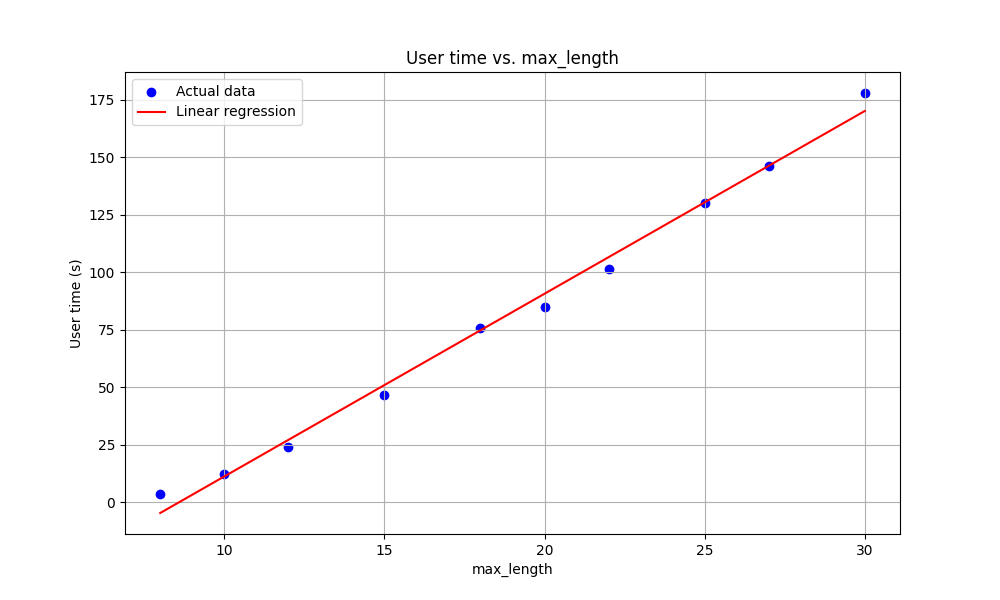
\includegraphics[scale=0.35]{user time vs max_length.png}}
\caption{User time vs. max\_length}
\label{fig}
\end{figure}

The corresponding equation is: $\text{time} = 7.953 \times \text{max\_length} - 68.413$, with a determination coefficient $R^2 = 0.9932$.\\
Thus, the influence of $\text{max\_length}$ on MAWs computation time is linear.

\subsection{Influence of Sequence Length on MAWs Computation}
We compute the MAWs for several sequences of different lengths, using a fixed $\text{max\_length}$ of 30.\\
The obtained results are:\\\\

\begin{table}[htbp]
\caption{Influence of Sequence Length on MAWs Computation}
\begin{center}
\begin{tabular}{|c|c|}
\hline
$\mathbf{|S|}$ & \textbf{User Time} \\
\hline
$1,022$ & $0$m$1.708$s\\
\hline
$2,467$ & $0$m$3.211$s\\
\hline
$3,828$ & $0$m$5.346$s\\
\hline
$7,005$ & $0$m$9.341$s\\
\hline
$10,031$ & $0$m$12.465$s\\
\hline
$15,398$ & $0$m$20.273$s\\
\hline
$25,014$ & $0$m$32.328$s\\
\hline
$50,100$ & $1$m$7.120$s\\
\hline
$100,021$ & $2$m$22.317$s\\
\hline
$200,231$ & $4$m$25.720$s\\
\hline
\end{tabular}
\end{center}
\end{table}

\begin{figure}[htbp]
\centerline{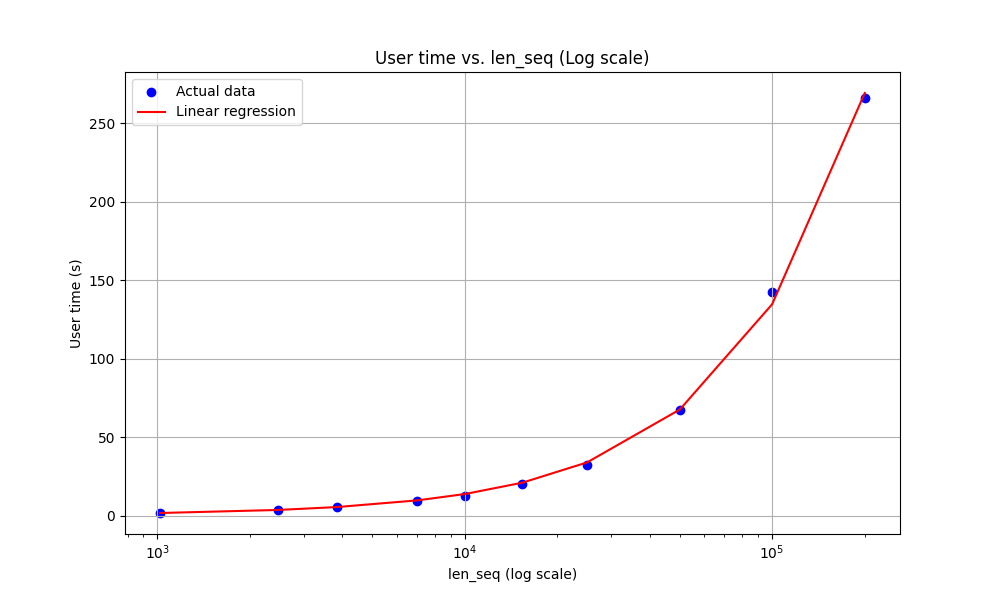
\includegraphics[scale=0.35]{user time vs len_seq(log scale).png}}
\caption{User time vs. Sequence Length (log scale)}
\label{fig}
\end{figure}

The corresponding equation is: $\text{time} = 0.001343 \times |S| + 0.223761$, with a determination coefficient $R^2 = 0.9988$.\\
Thus, the influence of sequence length on MAWs computation time is linear.
\subsection{Optimal $\text{max\_length}$}
From the previous experiments, we observe that $\text{max\_length}$ has a significant impact. Therefore, we aim to determine the value that optimally balances the number of captured MAWs and computation time.\\
Using high values, as in the second experiment, we identify the $\text{max\_length}$ that captures more than 99.9\% of MAWs. We choose such a high percentage because the distribution of MAWs follows a bell curve.\\
This is evident in the following graphs, both in linear and logarithmic scales, for sequences of length 200,000 bases:
\begin{figure}[htbp]
\centerline{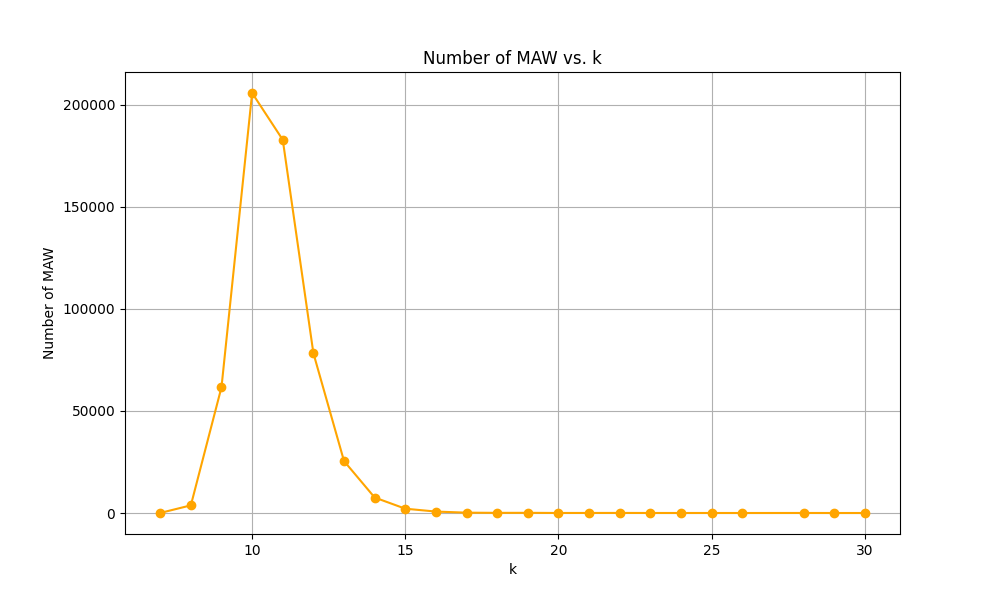
\includegraphics[scale=0.30]{number of MAW vs k.png}}
\caption{Number of MAWs vs. $k$}
\label{fig}
\end{figure}

\begin{figure}[htbp]
\centerline{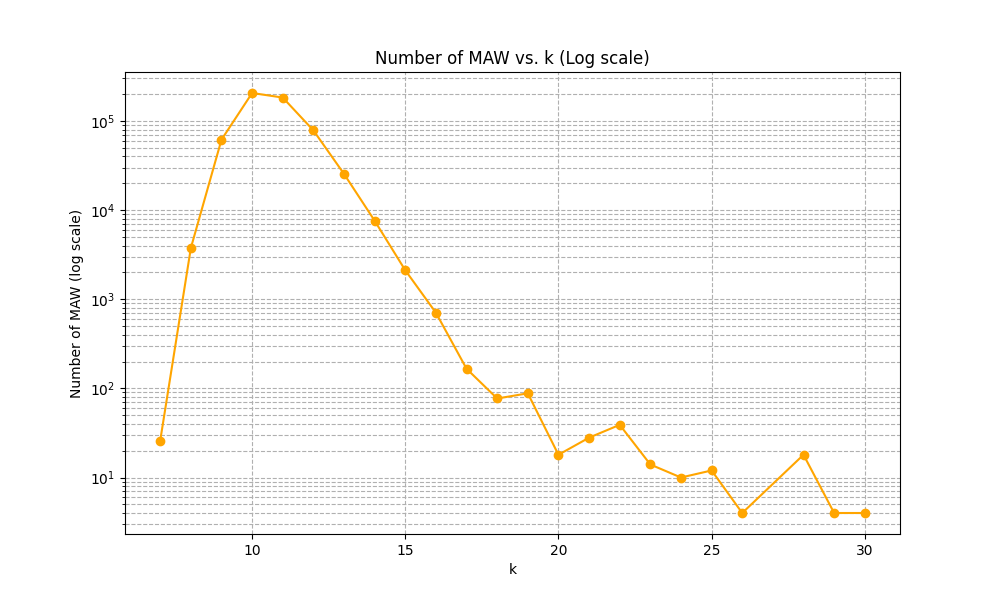
\includegraphics[scale=0.30]{number of MAW vs k (log scale).png}}
\caption{Number of MAWs vs. $k$ (log scale)}
\label{fig}
\end{figure}
$\quad$\\
\\
\\
\\
\\
\\
\\
\\
\\
\\


The results are summarized in the table below:

\begin{table}[htbp]
\caption{Optimal $\text{max\_length}$ for Capturing 99.9\% of MAWs}
\begin{center}
\begin{tabular}{|c|c|}
\hline
$\mathbf{|S|}$ & \textbf{Optimal max\_length} \\
\hline
$1,022$ & $13$\\
\hline
$2,467$ & $14$\\
\hline
$3,828$ & $19$\\
\hline
$7,005$ & $22$\\
\hline
$10,031$ & $16$\\
\hline
$15,398$ & $14$\\
\hline
$25,014$ & $18$\\
\hline
$50,100$ & $16$\\
\hline
$100,021$ & $16$\\
\hline
$200,231$ & $16$\\
\hline
\end{tabular}
\end{center}
\end{table}

We thus choose $\text{max\_length} = 20$ as the optimal value.

\subsection{Influence of $p$ on $p$-MAWs Computation}
We reuse the previous experiments to evaluate the influence of $p$.\\
We fix $\text{max\_length}$ to 20 and consider the first 10 sequences from the database (134,764 bases). We first compute the MAWs, then the $p$-MAWs for varying $p$.\\
The results are as follows:\\
\\
\\


\begin{table}[htbp]
\caption{Influence of $p$ on $p$-MAWs Computation}
\begin{center}
\begin{tabular}{|c|c|}
\hline
$\mathbf{p}$ & \textbf{User Time} \\
\hline
$0.3$ & $0$m$13.544$s\\
\hline
$0.4$ & $0$m$13.444$s\\
\hline
$0.5$ & $0$m$13.949$s\\
\hline
$0.6$ & $0$m$14.133$s\\
\hline
$0.7$ & $0$m$13.555$s\\
\hline
$0.8$ & $0$m$13.994$s\\
\hline
$0.9$ & $0$m$21.993$s\\
\hline
\end{tabular}
\end{center}
\end{table}

\subsection{Experimental Evaluation of $\gamma_p$ and $\delta_p$}
Under the same conditions as the previous experiment, we experimentally evaluate the two parameters.\\
The results are as follows:

\begin{table}[htbp]
\caption{Experimental Values of $\gamma_p$ and $\delta_p$}
\begin{center}
\begin{tabular}{|c|c|c|}
\hline
$\mathbf{p}$ & $\mathbf{\gamma_p}$ & $\mathbf{\delta_p}$ \\
\hline
$0.3$ & $0.01$ & $0.77$ \\
\hline
$0.4$ & $0.02$ & $0.65$ \\
\hline
$0.5$ & $0.03$ & $0.56$ \\
\hline
$0.6$ & $0.06$ & $0.52$ \\
\hline
$0.7$ & $0.12$ & $0.48$ \\
\hline
$0.8$ & $0.23$ & $0.45$ \\
\hline
$0.9$ & $0.43$ & $0.42$ \\
\hline
\end{tabular}
\end{center}
\end{table}

From both experiments, we observe that $p$ influences $\gamma_p$ and $\delta_p$. As $p$ approaches 1, $\gamma_p$ increases while $\delta_p$ decreases.\\
Thus, $p$ has a (slight) impact on computation time through the two parameters.\\
However, we note that $4 \times \gamma_p \times \delta_p$ remains well below 1 (for instance, it is 0.23 for $p = 0.7$), indicating that the computation does not enter an exponential regime.

\section{Discussion}
The experiments conducted show a linear influence of both sequence length and maximum motif size $\text{max\_length}$ on the computation time of MAWs. These results confirm the theoretical analyses presented in the methods section. However, some aspects need to be further explored and optimized. Notably, we observed in practice a complexity depending on $\text{max\_length}$, while the worst-case scenario theoretically depends on $\text{max\_length}^2$. It would be interesting to identify the conditions under which the worst-case complexity is reached.\\

Further work is required to eliminate more redundant computations during the search for $p$-MAWs. Although the implementation of a caching mechanism has limited some repetitive calculations, a more efficient data structure or a more optimized filtering method could further reduce these redundancies. This approach is particularly promising for improving algorithm performance on large sequence datasets or with high \textit{max\_length} values.\\

Additionally, the experimental evaluation of the parameters $\gamma_p$ and $\delta_p$ shows that these values vary depending on the threshold $p$. However, a more in-depth theoretical analysis is needed to establish precise bounds and, if possible, demonstrate that $4\gamma_p\delta_p$ is less than $1$, thus avoiding exponential complexity (at least for a reasonably chosen $p$).\\

Future work should focus on improving the verification step for $p$-MAWs and conducting a more thorough theoretical analysis of the parameters introduced in this study.

\begin{thebibliography}{00}
\bibitem{b1} F. Mojica, C. Diez-Villase\~nor, E. Soria, and G. Juez, ``Biological significance of a family of regularly spaced repeats in the genomes or Archæa, Bacteria and mitochondria``, in Molecular Microbiology, vol. 36, april 2000, pp. 244-246
\bibitem{b2} https://github.com/AlexeyG/PySAIS
\bibitem{b3}  G. Nong, S. Zhang, and W. H. Chan, ``Linear suffix array construction by almost pure induced-sorting``, in 2009 data compression conference, pp. 193-202, IEEE
\bibitem{b5} https://pypi.org/project/suffix-tree/
\bibitem{b6} E. Ukkonen, ``On-line construction of suffix trees``, in Algorithmica, vol. 14, no 3, 1995, pp. 249-260
\bibitem{b4} https://t.ly/uXirO
\end{thebibliography}
\end{document}
